\chapter{Bones and Muscles}\label{ch:g3:bones-and-muscles}

Jump, and land: something inside you just worked like a perfect
machine. Rigid rods held your shape, hinges let your \omterm{def:g1:my-body:parts}{legs} fold
and spring, and hundreds of little motors pulled exactly when
needed. The rods are your \omterm{def:g3:bones-and-muscles:skeleton}{bones}, the hinges your \omterm{prop:g3:bones-and-muscles:joints}{joints}, the
motors your \omterm{def:g3:bones-and-muscles:muscle}{muscles} --- the body's equipment for every movement
it will ever make.

\section{The skeleton}

\begin{definition}[Skeleton and bones]\label{def:g3:bones-and-muscles:skeleton}
The \emph{skeleton}\index{skeleton} is the frame of about $200$
\emph{bones}\index{bone} inside the body. Its main regions:
\begin{itemize}
  \item the \emph{skull}\index{skull}, a solid helmet of bone
        around the brain;
  \item the \emph{spine}\index{spine} (backbone), a bendable
        column of small bones stacked from neck to hips, holding
        the trunk upright;
  \item the \emph{ribs}\index{rib}, curved bones forming a cage
        around heart and lungs;
  \item the \emph{\omterm{def:g1:my-body:parts}{limb} bones}: long bones in \omterm{def:g1:my-body:parts}{arms} and \omterm{def:g1:my-body:parts}{legs} ---
        the thigh bone is the longest of the body.
\end{itemize}
\end{definition}

\begin{omfigure}
\begin{tikzpicture}
  \node[anchor=south west, inner sep=0] (img) at (0,0)
    {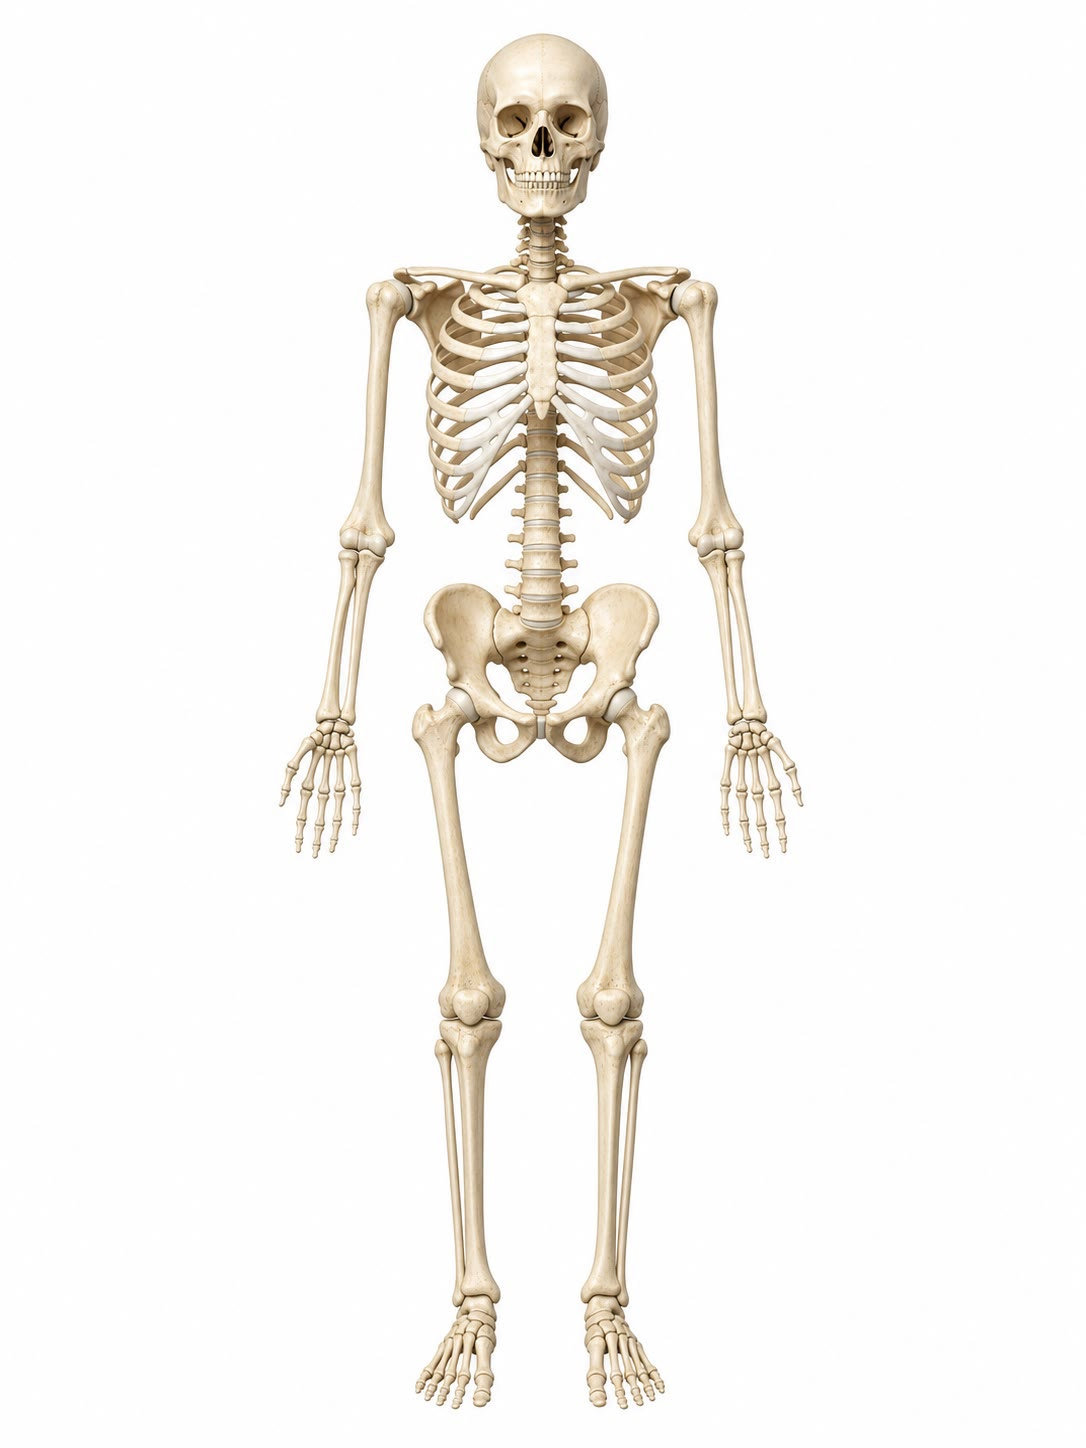
\includegraphics[width=0.46\linewidth]{images/book1/ai/fig-skeleton.jpg}};
  \begin{scope}[x={(img.south east)}, y={(img.north west)},
      every node/.style={font=\small}]
    \draw[omDef, thick] (0.56,0.93) -- (0.72,0.95) node[right] {skull};
    \draw[omDef, thick] (0.40,0.73) -- (0.20,0.82)
      node[above, align=center] {ribs: a cage for\\ heart and lungs};
    \draw[omDef, thick] (0.52,0.56) -- (0.72,0.60)
      node[right, align=left] {spine: stacked\\ small bones};
    \draw[omDef, thick] (0.60,0.36) -- (0.76,0.38) node[right] {thigh bone};
    \draw[omThm, thick] (0.335,0.615) circle (0.022);
    \draw[omThm, thick] (0.445,0.265) circle (0.022);
    \draw[omThm, thick] (0.425,0.265) -- (0.20,0.22)
      node[left, align=center, omThm] {joints (in red):\\ where bones meet};
  \end{scope}
\end{tikzpicture}

{\small The \omterm{def:g3:bones-and-muscles:skeleton}{skeleton}'s plan: helmet, column, cage, and long \omterm{def:g1:my-body:parts}{limb}
\omterm{def:g3:bones-and-muscles:skeleton}{bones} meeting at \omterm{prop:g3:bones-and-muscles:joints}{joints}.}
\end{omfigure}

\begin{example}[Feel your frame]\label{ex:g3:bones-and-muscles:feel}
No X-ray needed: press gently and the \omterm{def:g3:bones-and-muscles:skeleton}{skeleton} reports. Knuckles;
the ridge of the shin; the chain of small bumps down the middle
of your back --- the \omterm{def:g3:bones-and-muscles:skeleton}{spine}, one small \omterm{def:g3:bones-and-muscles:skeleton}{bone} after another; the
\omterm{def:g3:bones-and-muscles:skeleton}{ribs} you can count under your fingers. The frame is right under
the \omterm{def:g1:the-five-senses:sense}{skin}.
\end{example}

\begin{remark}[Hard outside, alive inside]\label{rem:g3:bones-and-muscles:alive}
A \omterm{def:g3:bones-and-muscles:skeleton}{bone} is not dead material like a chalk stick: it is living, fed
by blood, growing while you grow --- and able to repair itself.
A broken \omterm{def:g1:my-body:parts}{arm} in a cast mends because the \omterm{def:g3:bones-and-muscles:skeleton}{bone} itself slowly
rebuilds the break. Chalk sticks never do that.
\end{remark}

\begin{omfigure}
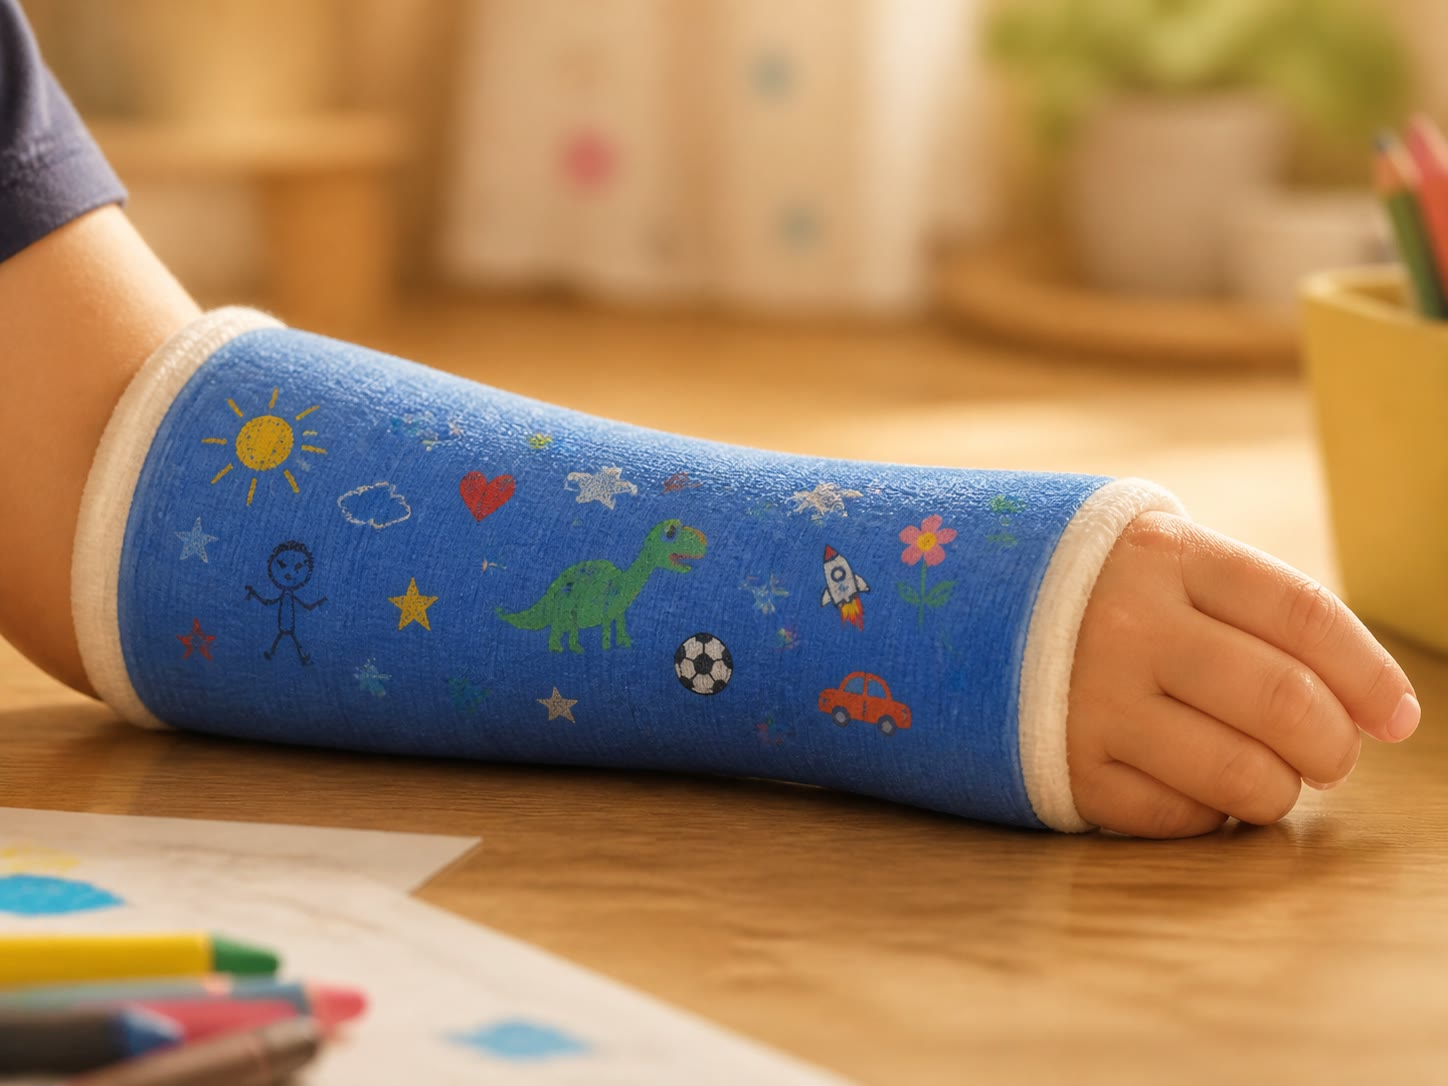
\includegraphics[width=0.56\linewidth]{images/book1/ai/g3-bones-cast.jpg}

{\small Inside the decorated cast, held still, a living \omterm{def:g3:bones-and-muscles:skeleton}{bone} is
quietly rebuilding itself.}
\end{omfigure}

\section{Joints, where the frame bends}

\begin{proposition}[Rigid rods, bending places]\label{prop:g3:bones-and-muscles:joints}
\omterm{def:g3:bones-and-muscles:skeleton}{Bones} themselves never bend --- a bent \omterm{def:g3:bones-and-muscles:skeleton}{bone} is a broken \omterm{def:g3:bones-and-muscles:skeleton}{bone}.
All the body's bending happens at the
\emph{joints}\index{joint}, where two \omterm{def:g3:bones-and-muscles:skeleton}{bones} meet: \omterm{def:g1:my-body:joint}{shoulder},
\omterm{def:g1:my-body:joint}{elbow}, \omterm{def:g1:my-body:joint}{wrist}, hip, \omterm{def:g1:my-body:joint}{knee}, \omterm{def:g1:my-body:joint}{ankle}, and the many small \omterm{prop:g3:bones-and-muscles:joints}{joints} of the
\omterm{def:g3:bones-and-muscles:skeleton}{spine}, whose little bends add up to a supple back.
\end{proposition}
\admitted

\begin{example}[The spine's trick]\label{ex:g3:bones-and-muscles:spinetrick}
No single \omterm{def:g3:bones-and-muscles:skeleton}{bone} in your back can curl --- yet you can roll
forward almost into a ball. The \omterm{def:g3:bones-and-muscles:skeleton}{spine} is a column of more than
$20$ small \omterm{def:g3:bones-and-muscles:skeleton}{bones}, each turning a few degrees on its neighbors:
many small bends making one big one. That is also why you should
bend \omterm{def:g1:my-body:joint}{knees}, not back, to lift something heavy --- \omterm{def:g1:my-body:joint}{knees} are
built for big folds, the \omterm{def:g3:bones-and-muscles:skeleton}{spine} for gentle ones.
\end{example}

\section{Muscles, the movers}

\begin{definition}[Muscle]\label{def:g3:bones-and-muscles:muscle}
A \emph{muscle}\index{muscle} is a fleshy motor attached to the
\omterm{def:g3:bones-and-muscles:skeleton}{bones}. A muscle can \emph{contract}\index{contract} --- shorten
and thicken --- and in contracting it \emph{pulls} the \omterm{def:g3:bones-and-muscles:skeleton}{bone} it
is attached to. Muscles only pull; no muscle can push.
\end{definition}

\begin{proposition}[Working in pairs]\label{prop:g3:bones-and-muscles:pairs}
Since \omterm{def:g3:bones-and-muscles:muscle}{muscles} only pull, moving a \omterm{def:g1:my-body:joint}{joint} both ways takes a
\emph{pair}: one \omterm{def:g3:bones-and-muscles:muscle}{muscle} in front of the \omterm{def:g1:my-body:parts}{arm} bends the \omterm{def:g1:my-body:joint}{elbow}, its
partner behind straightens it; each relaxes while the other
pulls. Nearly every \omterm{def:g1:my-body:joint}{joint} of the body is moved by such pairs.
\end{proposition}
\admitted

\begin{omfigure}
\begin{tikzpicture}
  \node[anchor=south west, inner sep=0] (img) at (0,0)
    {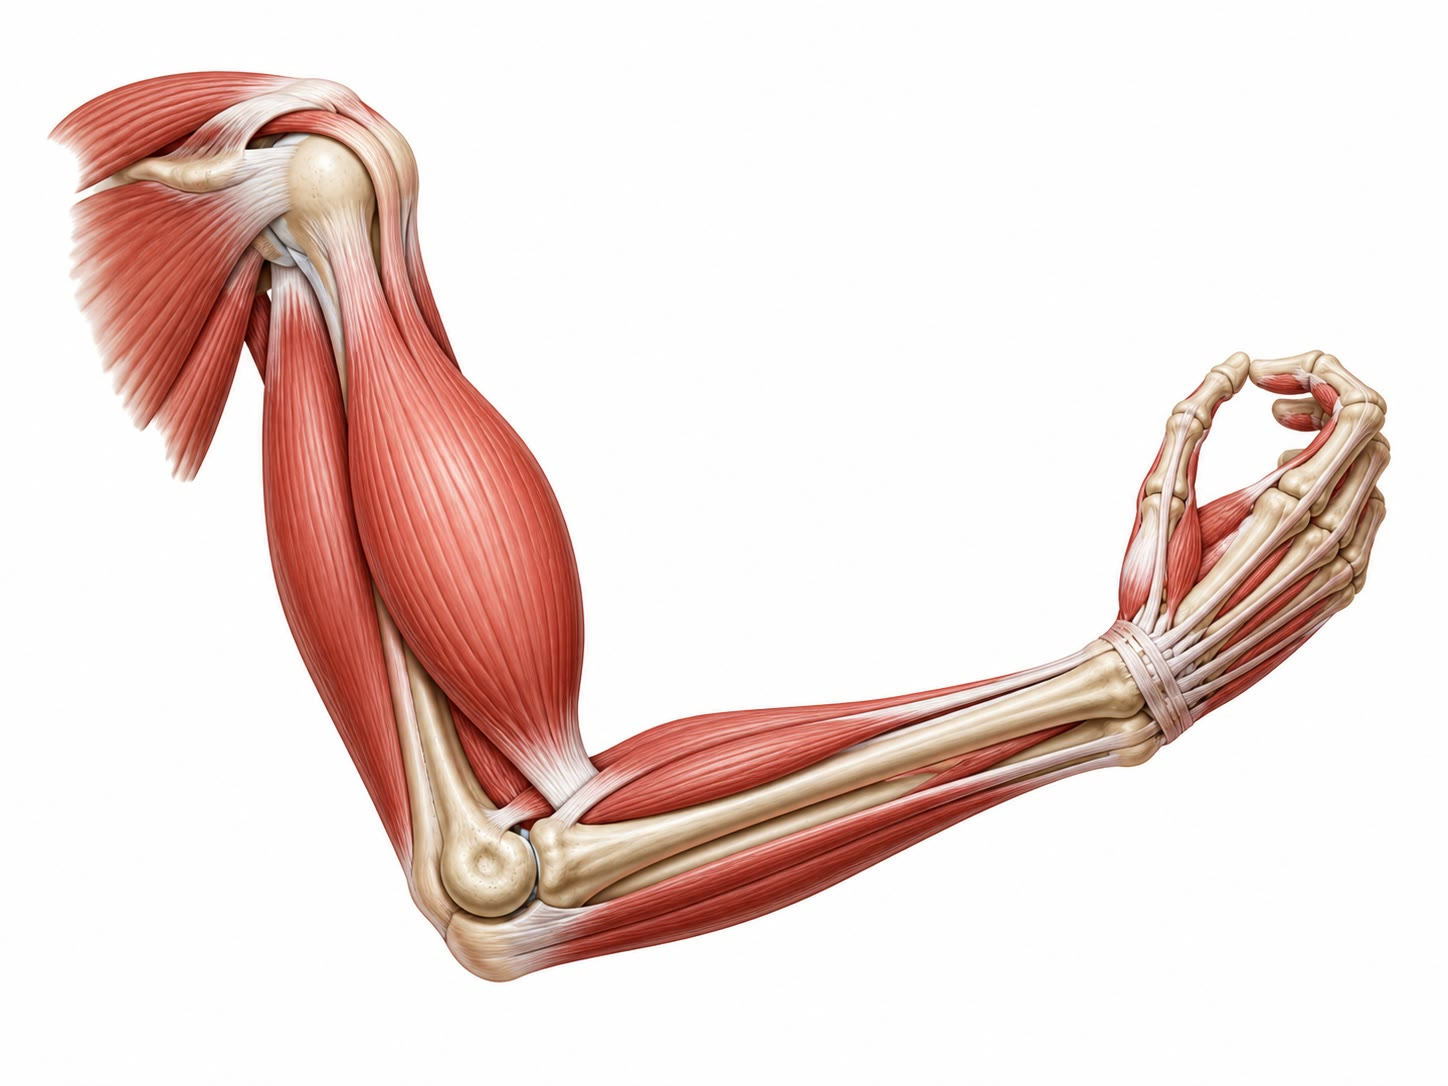
\includegraphics[width=0.62\linewidth]{images/book1/ai/fig-arm-muscles.jpg}};
  \begin{scope}[x={(img.south east)}, y={(img.north west)},
      every node/.style={font=\small}]
    \draw[omThm, thick] (0.42,0.58) -- (0.58,0.78)
      node[right, align=left, omThm]
      {the front muscle, bulging:\\ it contracts and pulls};
    \draw[omDef, thick] (0.23,0.46) -- (0.14,0.22)
      node[below, align=center, omDef]
      {the back muscle\\ of the pair, resting};
  \end{scope}
\end{tikzpicture}

{\small Bending the \omterm{def:g1:my-body:joint}{elbow}: the front \omterm{def:g3:bones-and-muscles:muscle}{muscle} of the pair bulges as
it shortens and pulls the forearm up, while its partner behind
rests. To straighten, the two swap roles.}
\end{omfigure}

\begin{example}[Feel the pair at work]\label{ex:g3:bones-and-muscles:pair}
Grip your upper \omterm{def:g1:my-body:parts}{arm} with the other hand and slowly bend the
\omterm{def:g1:my-body:joint}{elbow}: the \omterm{def:g3:bones-and-muscles:muscle}{muscle} in front swells and hardens --- it is
contracting. Now straighten the \omterm{def:g1:my-body:parts}{arm}: the front softens, and
behind the \omterm{def:g1:my-body:parts}{arm} its partner tightens instead. You have just felt
\cref{prop:g3:bones-and-muscles:pairs} happen.
\end{example}

\begin{method}[Looking after bones and muscles]\label{met:g3:bones-and-muscles:care}
\begin{enumerate}
  \item Move every day --- \omterm{def:g3:bones-and-muscles:skeleton}{bones} grow stronger, \omterm{def:g3:bones-and-muscles:muscle}{muscles} too, with
        use;
  \item eat the builders' foods: dairy for \omterm{def:g3:bones-and-muscles:skeleton}{bones}, and varied
        meals (\cref{ch:g2:teeth-and-eating-well});
  \item warm up before hard exercise, so \omterm{def:g3:bones-and-muscles:muscle}{muscles} stretch instead
        of tearing;
  \item lift heavy things with bent \omterm{def:g1:my-body:joint}{knees} and a straight back;
  \item helmets and pads where falls are likely: \omterm{def:g3:bones-and-muscles:skeleton}{bones} repair,
        but slowly.
\end{enumerate}
\end{method}

\section{Exercises}

\begin{exercise}[$\star$]\label{exo:g3:bones-and-muscles:1}
Name the four regions of the \omterm{def:g3:bones-and-muscles:skeleton}{skeleton} in
\cref{def:g3:bones-and-muscles:skeleton}, and what each
protects or holds up.
\end{exercise}

\begin{exercise}[$\star$]\label{exo:g3:bones-and-muscles:2}
About how many \omterm{def:g3:bones-and-muscles:skeleton}{bones} has the \omterm{def:g3:bones-and-muscles:skeleton}{skeleton}? Which is the longest?
\end{exercise}

\begin{exercise}[$\star$]\label{exo:g3:bones-and-muscles:3}
Can a \omterm{def:g3:bones-and-muscles:skeleton}{bone} bend? Where does all the body's bending happen?
\end{exercise}

\begin{exercise}[$\star$]\label{exo:g3:bones-and-muscles:4}
The \omterm{def:g3:bones-and-muscles:skeleton}{spine} can curl although none of its \omterm{def:g3:bones-and-muscles:skeleton}{bones} can. Explain its
trick.
\end{exercise}

\begin{exercise}[$\star$]\label{exo:g3:bones-and-muscles:5}
What does a \omterm{def:g3:bones-and-muscles:muscle}{muscle} do when it \omterm{def:g3:bones-and-muscles:muscle}{contracts}? What can no \omterm{def:g3:bones-and-muscles:muscle}{muscle}
ever do?
\end{exercise}

\begin{exercise}[$\star$]\label{exo:g3:bones-and-muscles:6}
Why does bending and straightening the \omterm{def:g1:my-body:joint}{elbow} need two \omterm{def:g3:bones-and-muscles:muscle}{muscles}?
Tell what each does at each moment.
\end{exercise}

\begin{exercise}[$\star$]\label{exo:g3:bones-and-muscles:7}
How does a broken \omterm{def:g1:my-body:parts}{arm} in a cast mend? What does this show about
\omterm{def:g3:bones-and-muscles:skeleton}{bone}, by \cref{rem:g3:bones-and-muscles:alive}?
\end{exercise}

\begin{exercise}[$\star$]\label{exo:g3:bones-and-muscles:8}
Try it: do the grip test of \cref{ex:g3:bones-and-muscles:pair}
on your own \omterm{def:g1:my-body:parts}{arm}. Describe what the front of the \omterm{def:g1:my-body:parts}{arm} does when
you bend, and when you straighten.
\end{exercise}

\begin{exercise}[$\star\star$]\label{exo:g3:bones-and-muscles:9}
Why do grown-ups say ``lift with your \omterm{def:g1:my-body:joint}{knees}, not with your
back''? Answer with \cref{ex:g3:bones-and-muscles:spinetrick}.
\end{exercise}

\begin{exercise}[$\star\star$]\label{exo:g3:bones-and-muscles:10}
A puppet on strings can be made to wave: each string can only
\emph{pull} its \omterm{def:g1:my-body:parts}{arm} one way. How is this exactly the \omterm{def:g3:bones-and-muscles:muscle}{muscles}'
situation, and what is the puppet-maker's answer to it?
Compare with \cref{prop:g3:bones-and-muscles:pairs}.
\end{exercise}
